\documentclass[12pt,letterpaper]{article}
\usepackage[utf8]{inputenc}

\usepackage{graphicx}
\setlength{\parskip}{1em}
\setlength{\parindent}{0em}

\begin{document}
\title{
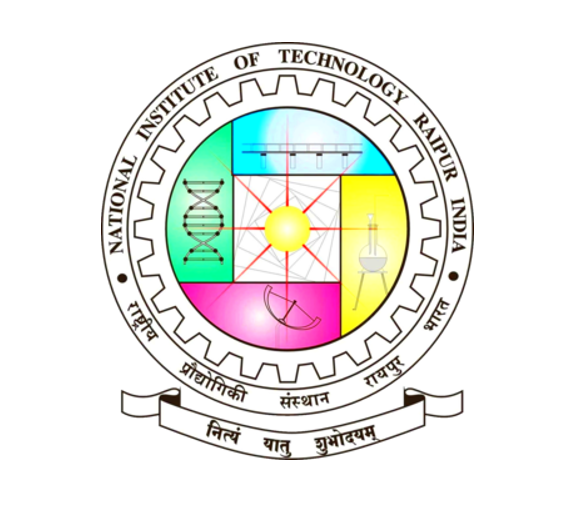
\includegraphics[width=0.3\textwidth]{National_Institute_of_Technology,_Raipur_Logo.png}
 \\ 
Philosophy of Artificial Intelligence
}

\author{SHREEDUTT 19111056 BME 5TH SEMESTER}

\maketitle
\rule{\textwidth}{0.5pt}
\begin{Summary}

    \noindent Synthetic blood vessels are beginning to resemble actual blood vessels. According to new
studies, “bioengineered” blood vessels will incorporate living cells after being inserted in the
human body, transforming them into blood-carrying, self-healing tubes that act more like human
blood vessels than alternatives. Blood vessels are a type of soft tissue that do not follow
Hooke's Law. In this article we will look at some properties of synthetic blood vessels and how
this will change the Human future in Testing and Curing of various diseases. The study is based
on a biomechanical model of a Synthetic blood vessel.The perfect vascular graft is made up of
Synthetic blood vessels made of viable tissue. The ability to regenerate, remodel, contract, and
secrete normal blood vessel products, as well as the lack of thrombogenicity and infection
tolerance, are all theoretical advantages of such grafts. A structural scaffold made of collagen or
a biodegradable polymer, vascular cells, and a nurturing environment are typically needed for
the construction of an artificial vessel. Bioreactors that produce pulsatile flow mimic the in vivo
environment of vascular cells, improving the mechanical properties of artificial vessels.
    
\end{abstract}
\rule{\textwidth}{0.5pt}

TABLE OF CONTENT\\
\rule{\textwidth}{0.5pt}
1) Introduction.\\
2) Background
\\
3) Requirement of Mechanical Properties of Synthetic Blood Vessels.\\
4) Components of blood vessel\\
5) Translational challenges\\
6) Conclusion.\\
7) References.\\

\section{Introduction}
  Cardiovascular disease (CVD) affects more than 71 million people in the United States alone,
with estimated costs exceeding 500 billion dollar. In America, the number of annual inpatient visits for
cardiovascular disease was over 7 million, with over 450,000 in-patient bypass procedures,
owing in part to failure. Finally, the failure of synthetic grafts to expand and adapt limits their
usefulness in paediatric patients.Due to this there is a huge need of concept will closely match
the biomechanical aspects of healthy artery and be capable of growth, remodeling, and
vasoactive responses.The demand is increasing for synthetic blood vessels to treat diseases such as those affecting
the heart and blood vessels of elderly and middle-aged patients. Due to the current shift in the
demographic structure caused by an aging society, the prospect for Artificial ones seems to be
very bright. Our society’s concerns regarding health are intensifying due to recent global trends
toward aging demographics, increase of adult diseases, increase of diseases due to
environmental pollution, and the emergence of new viruses. In recent years, there has been a
strong emphasis on the importance of prevention and treatment through diagnosis. As the
paradigm shifts to wellness, it
is expected that the demand for advanced fusion diagnosis and medical devices for treatment
will increase.
Tissue engineering has become a modern method for tissue regeneration by seeding functional
cells on biodegradable scaffolds. There has been significant progress in the field of vascular
engineering since Weinberg and Bell announced the in vitro construction of blood vessels using
collagen and cultured bovine aortic endothelial cells, smooth muscle cells, and adventitial
fibroblasts. Tissue-engineered blood vessels (TEBVs) have so far been successfully designed in
vitro and used to repair vascular defects in animal models. Just a few people have had clinical
success with this method.
The aim of this review is to summarise the major advancements in the field, including seeding
cell sources, biodegradable scaffolds, construction methods, and promising clinical results. The
remaining issues will be addressed as well, in order to help direct future efforts
\section{Background}
As the population ages, the area of heart disease is one of the therapeutic areas where
prevention and treatment are important. Globally, heart disease has been a leading cause of
deaths of people aged 60 or older and the number of people with heart disease is increasing.
Therefore, the demand for medical devices for treating heart disease is expected to increase.
As of 2012, WHO estimates that 37% of deaths from non-communicable diseases are
attributable to heart disease and that cardiac mortality rates will increase from 17.5 million in
2012 to 22.2 million in 2030. According to the World Health Organization (WHO), it was
estimated that there were about 347 million diabetics in 2014 and the risk of heart disease
resulting in death reaches 42% as the blood glucose levels rise.
As individuals age, the blood vessels that supply oxygen and nutrients to vital organs such as
the brain or heart become clogged up. The most common heart disease is myocardial infarction,
which is a clogging of the heart arteries, and angina, which narrows the heart arteries. All of
them are emergency medical illnesses associated with sudden death. Symptoms should be
treated within 6 to 12 h after the onset of symptoms. In this case, the most commonly used
procedure is coronary intervention on arteries which lead to the legs. It is a procedure to insert a
cardiovascular stenosis into a blocked part using a metal wire net stent or . The demand is
increasing to treat diseases such as those affecting the heart and blood vessels of elderly and
middle-aged people. Due to the current shift in the demographic structure caused by the aging
of society, the prospect for stents seems to be very bright. The vascular stent market accounts
for approximately 98.7 percent  7.65 billion of the total market (vascular and the non-vascular), andthe increase of vascular disease is expected to generate continuous demand in the Synthetic
Blood vessel market
\section{ Requirement of Mechanical Properties of Synthetic Bl }
Tissue engineering usually begins with seeding cells on biodegradable scaffolds, followed by in
vitro culture or in vivo implantation. The scaffolds should, in theory, be gradually resorbed,
leaving only the new tissue produced by the cells. Seeding cells, scaffolds, and construction
technologies all play a role in effective tissue regeneration.
Non-thrombogenic, non-immunogenic, consistent with high blood flow rates, and comparable
viscoelasticity to native vessels are all requirements for functional TEBVs. Furthermore, the
grafts should be living tissues that can gradually blend in with the body and blend in with the
native vessels. It has been approved

\section{Component of Blood Vessel}
The mechanics of blood vessel are mainly governed by type I and type III collagen fibres,
elastin, proteoglycan, and Smooth Muscle Cells concentration and orientation. But the relation
that we obtain between the collagen fiber and elastin shows some puzzling result which may not
be considered as accurate hence much research work needs to be done on this area.
The tunica intima, tunica media, and tunica adventitia are the three layers of blood vessels,
which are called from the luminal side outward. The thickness of these three layers varies
significantly depending on the size and form of artery (large, medium, and small arteries and
veins have three layers; capillaries do not).
The vascular wall except for capillaries is made up of three types of cells: endothelial cells that
line the tunica intima, smooth muscle cells that line the tunica media, and adventitial fibroblasts
that line the tunica adventitia.The endothelium layer serves as a thrombo-resistant, continuous
selective permeable barrier that allows for laminar blood flow through the blood vessel. It also
regulates leukocyte adhesion and proliferation, as well as platelet activation, adhesion, and
aggregation. SMCs, on the other hand, have secrecy. The SMCs secrete collagen fibres, elastic
fibres, elastic lamellae, and proteoglycans that keep the vessel's elasticity and radial
enforcement.

\section{Translational Challenge}
For paediatric pulmonary artery replacement, TEBV has needed at least a bone marrow
aspiration and brief cell seeding, as well as up to 28 weeks of maturation of rolled fibroblast
sheets to withstand arterial pressures for use as arteriovenous conduits in dialysis patients. The
next generation of solutions could be powered by advanced cell or biomaterial technologies.
The recent discovery that BMCs are only likely to live for a short time and that cellular
repopulation is triggered by monocyte infiltration could lead to new cell and biomaterial
strategies for TEBV researchers. In addition, preliminary findings relating biodegradablepolymer scaffold systems to the arterial system are promising. Furthermore, preliminary findings
in mice transferring biodegradable polymer scaffold systems to the arterial circulation indicate
that protocols requiring as little as one week of culture maturation may be feasible.


\section{Conclusion}
Engineering vessel grafts by seeding ECs on a proper biodegradable scaffold could be the best
way to facilitate the use of TEBVs in clinical application in the short term. In the long run, a
scaffold with antithrombogenic potential at an early stage and the ability to recruit ECs at later
stages is predicted. Other techniques, such as therapeutic gene delivery, have piqued
researchers' interest in tissue engineering. Pre-clinical human trials must be conducted in
immunocompetent large animal models, regardless of which method is taken, and long-term
results must be monitored.
The development of an immunologically humanised animal is necessary for such experiments.
Zeng et al. recently developed a goat model of human cells by implanting human cord blood
cells into foetal goats at 45–55 days of gestation. Human cells were found to have engrafted in
haematopoietic and non-haematopoietic organs for up to two years. The goat should have been
immunologically humanised so that it would not reject human cells in theory. Extensive research
is being carried out to back up the claims. Hopefully, this xeno-transplant goat can serve as a
one-of-a-kind model for evaluating engineered human tissue
\section{References}
1) Tissue engineering of blood vessel
Wen Jie Zhang, Wei Liu, Lei Cui, Yilin Cao\\
2) Analysis of trends and prospects regarding stents for human blood vessels
Jeong Hee Lee, Eung Do Kim, Eun Jung Jun, Hyoung Sun Yoo and Joon Woo Lee\\
3) Tissue Engineering of Blood Vessels: Functional Requirements,Progress, and Future
Challenges
VIVEK A. KUMAR, LUKE P. BREWSTER, JEFFREY M. CAVES and ELLIOT L.
CHAIKOF
\end{document}
